\section{Performance Evaluation and Metrics}\label{secperformance}
Evaluating the performance of computer vision tasks is far from trivial. They are typically categorized into four areas: image classification, object detection, semantic segmentation, and instance segmentation, each with distinct objectives. As a result, the performance metrics applicable to one category may not be suitable for another. Moreover, each segmentation task has unique requirements and deals with different types of images, which influences the relevance of performance metrics. In our work, we focus on binary instance segmentation for both myotube and cell nuclei images. Given the distinct characteristics of these image types, we selected a set of performance metrics that we believe most accurately reflect our model's performance.
Instance segmentation tasks fundamentally involve classification, where metrics gauge a model's ability to differentiate between categories using counts of true positives, false positives, and false negatives. In binary instance segmentation, true negatives, which would correspond to the image background, are not considered. We assess our models' detection quality through metrics like precision (the rate at which predicted instances are correctly classified), recall (the ability to identify all relevant instances), and accuracy (the average of precision and recall). We also employ overlap-based metrics to compare predictions with ground truths in images and to gauge our models' segmentation quality. Metrics such as Intersection over Union (IoU), Intersection over Reference (IoR), and Normalized Surface Distance (NSD) are used, depending on the image type. These metrics are calculated for matched true positive and ground truth instances and reported both before and after normalization by the number of ground truth masks. Additionally, we report Panoptic Quality, a hybrid metric that combines segmentation and detection quality into one, yielding more conservative results due to its multiplicative factors ranging from 0 to 1. An overview over the performance metrics can be obtained in Table~\ref{tabdefs}. More detailed explanations on the quantities can be found in \cite{metricsreloaded}.


\subsection{Performance Evaluation}
In the following two subsections, we present these metrics for \texttt{Stardist}, used to segment cell nuclei, and \texttt{MyoSAM}, our model for myotube segmentation. We also juxtapose the performance of \texttt{MyoSAM} to Meta’s \texttt{SAM} model for direct comparison.
\subsubsection{Performance of Cell Nuclei Segmentation with \texttt{Stardist}}

\begin{figure}
	\centering
	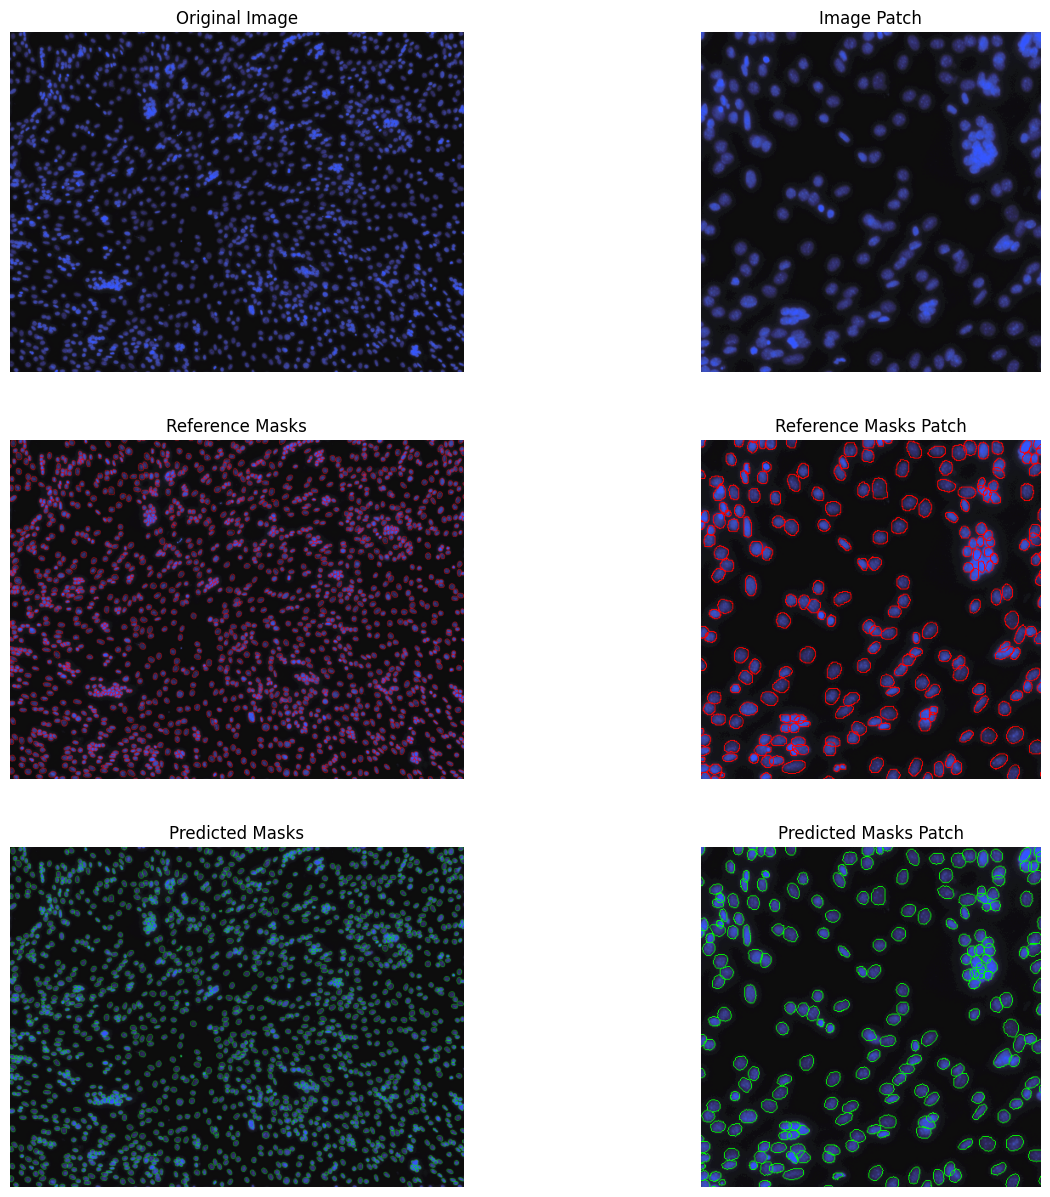
\includegraphics[width=\textwidth]{"images/qualitative_performance_stardist.png"}
	\caption[Qualitative performance \texttt{Stardist}]{Comparison of one sample image and one patch therein in terms of ground truth and \texttt{Stardist} prediction.}
	\label{figperfstardistqual}
\end{figure} 

Qualitatively, \texttt{Stardist} effectively segments cell nuclei, closely matching the shapes of manually annotated reference masks as can be seen from Fig.~\ref{figperfstardistqual}. Despite its generally precise segmentations, \texttt{Stardist} tends to slightly underestimate the number of nuclei in densely clustered areas. This observation is supported by the difference in number of reference masks ($n=1923$) compared to predicted masks ($n=1823$). To quantify this performance, we matched predictions with references using the Intersection over Reference metric, allowing less penalization for predictions that segment multiple references and accommodating single predictions to multiple references. Double assignments in matching are considered false positives.
The common threshold for mask matching in computer vision is $\tau = 0.5$, but this may be too conservative for small objects like cell nuclei, where minimal prediction shifts can noticeably impact overlap metrics. Despite this, \texttt{Stardist}'s performance remains robust even at conservative thresholds (cf. Fig.~\ref{figperfstardist} and Table~\ref{tabstardist}).


\begin{figure}
	\centering
	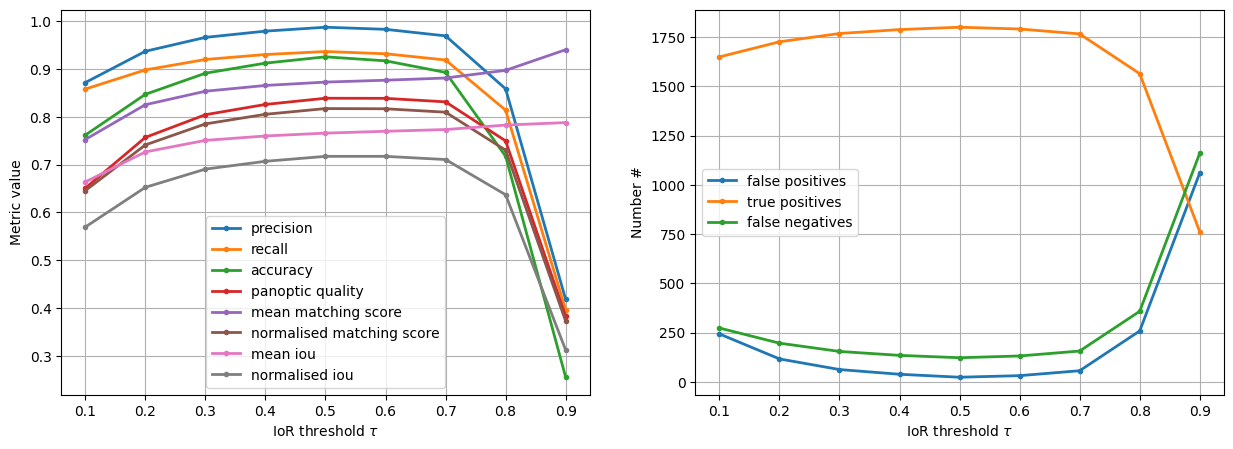
\includegraphics[width=\textwidth]{"images/quantitative_performance_stardist.png"}
	\caption[Quantitative performance \texttt{Stardist}]{Performance of \texttt{Stardist} in terms of the described metrics and ROC metrics.}
	\label{figperfstardist}
\end{figure} 

\begin{table}[H]
	\centering
	\caption{Stardist Performance ($\tau = 0.5$)}
	\label{tabstardist}
	\begin{tabular}{|l|c|}
		\hline
		True Positives & 1801 \\
		\hline
		False Positives & 23 \\
		\hline
		False Negatives & 122 \\
		\hline
		Precision & 0.99 \\
		\hline
		Recall & 0.94 \\
		\hline
		Accuracy & 0.93 \\
		\hline
		Panoptic Quality & 0.84 \\
		\hline
		Mean Matching Score (IoR) & 0.87 \\
		\hline
		Normalised Matching Score (IoR) & 0.82 \\
		\hline
		Mean IoU & 0.77 \\
		\hline
		Normalised IoU & 0.72 \\
		\hline
	\end{tabular}
\end{table}

\subsubsection{Performance of Myotube Segmentation with \texttt{MyoSAM}}

\begin{figure}
	\centering
	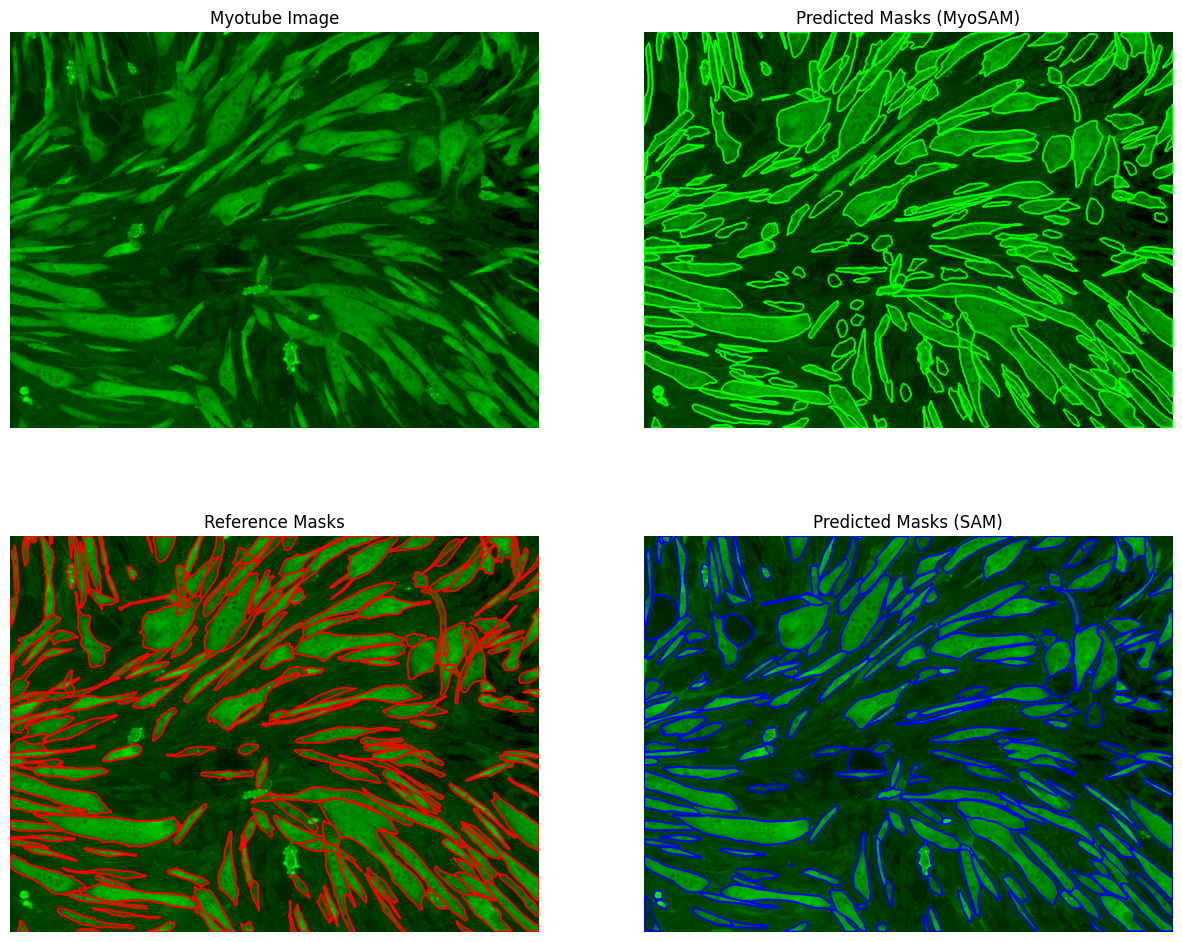
\includegraphics[width=\textwidth]{"images/qualitative_performance_myosam.png"}
	\caption[Qualitative performance \texttt{MyoSAM}]{Qualitative comparison of a myotube image with \texttt{SAM}, \texttt{MyoSAM}, and ground truth.}
	\label{figperfsamqual}
\end{figure} 
The performance comparison between \texttt{MyoSAM} and the standard \texttt{SAM} model highlights several key differences. Our focus with \texttt{MyoSAM} was on accurately delineating myotube boundaries, crucial for medical evaluations of microscopy images. To this end, we report the Normalized Surface Distance as an overlap metric for myotubes, which is a measure of overlap of the mask boundaries. NSD has an adjustable parameter $\tau_{\text{NSD}}$, with which the boundaries of both masks can be widened to account for inter-rater-variability. We set the parameter at three, meaning the boundaries were widened by three pixels both inward and outward.
Despite \texttt{SAM}'s capabilities, it faces challenges in accurately segmenting overlapping myotubes, often misidentifying them as separate entities or as disconnected parts of the same segment. Its design to segment a wide range of features results in the unnecessary segmentation of insignificant details, such as minor grains or shades within myotubes. Additionally, SAM sometimes generates redundant masks for a single myotube, a byproduct of its training to handle ambiguous prompts, despite there being no such ambiguity in myotube identification. This highlights the need for tailored approaches in myotube segmentation to avoid these specific issues. Our qualitative comparison in Fig.~\ref{figperfsamqual} shows \texttt{MyoSAM} significantly improves on these issues, but how do the metrics reflect this? We matched myotube references and predictions using IoU, and we recommend a matching threshold $\tau = 0.5$ due to the larger size of myotubes compared to nuclei. \texttt{MyoSAM} outperforms \texttt{SAM} in almost all aspects and every matching threshold except one and a slight increase in the number of predicted masks, demonstrating a quality over quantity advantage. Their individual performances are seen in Fig.~\ref{figperfsam} and Fig.~\ref{figperfsambase} while the improvement due to the training measured in terms of differences in performance metrics is seen in Fig.~\ref{figperfdiffsam}. A summary of the metrics for $\tau = 0.5$ can be found in Table~\ref{tabmyosamvssam}.
\begin{table}[H]
	\centering
	\caption{MyoSAM vs SAM ($\tau = 0.5$)}
	\label{tabmyosamvssam}
	\begin{tabular}{|l|c|c|c|}
		\hline
		Metric & MyoSAM & SAM & Difference \\
		\hline
		True Positives & 169 & 161 & 8.00 \\
		\hline
		False Positives & 65 & 69 & -4.00 \\
		\hline
		False Negatives & 43 & 51 & -8.00 \\
		\hline
		Precision & 0.72 & 0.7 & 0.02 \\
		\hline
		Recall & 0.79 & 0.76 & 0.03 \\
		\hline
		Accuracy & 0.61 & 0.57 & 0.04 \\
		\hline
		Panoptic Quality & 0.62 & 0.57 & 0.05 \\
		\hline
		Mean Matching Score & 0.81 & 0.78 & 0.03 \\
		\hline
		Normalised Matching Score & 0.65 & 0.59 & 0.06 \\
		\hline
		Mean NSD & 0.88 & 0.83 & 0.05 \\
		\hline
		Normalised NSD & 0.7 & 0.63 & 0.07 \\
		\hline
	\end{tabular}
\end{table}
\begin{figure}
	\centering
	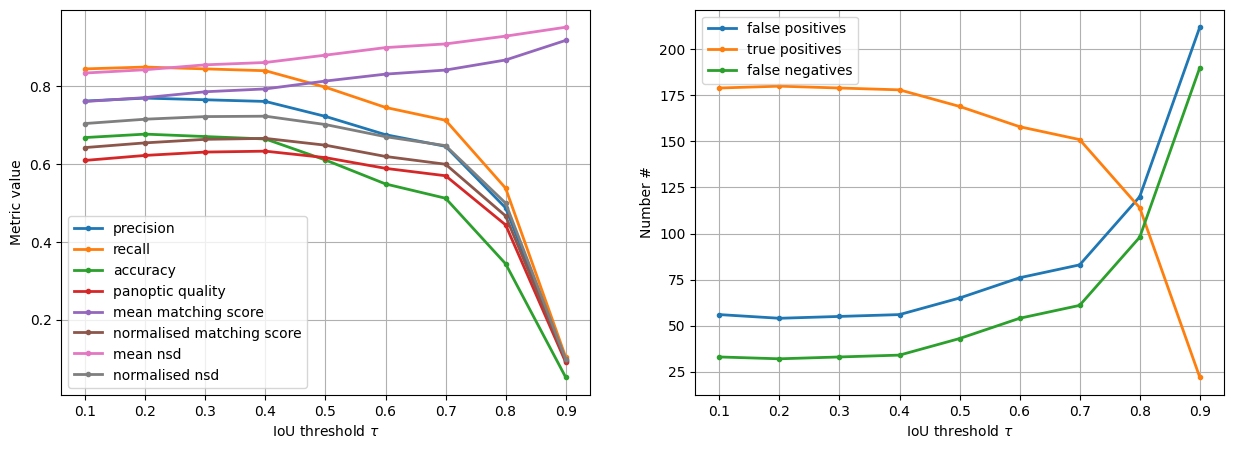
\includegraphics[width=\textwidth]{"images/quantitative_performance_myosam.png"}
	\caption[Quantitative performance \texttt{MyoSAM}]{Performance of \texttt{MyoSAM} in terms of the described metrics and ROC metrics.}
	\label{figperfsam}
\end{figure}
\begin{figure}
	\centering
	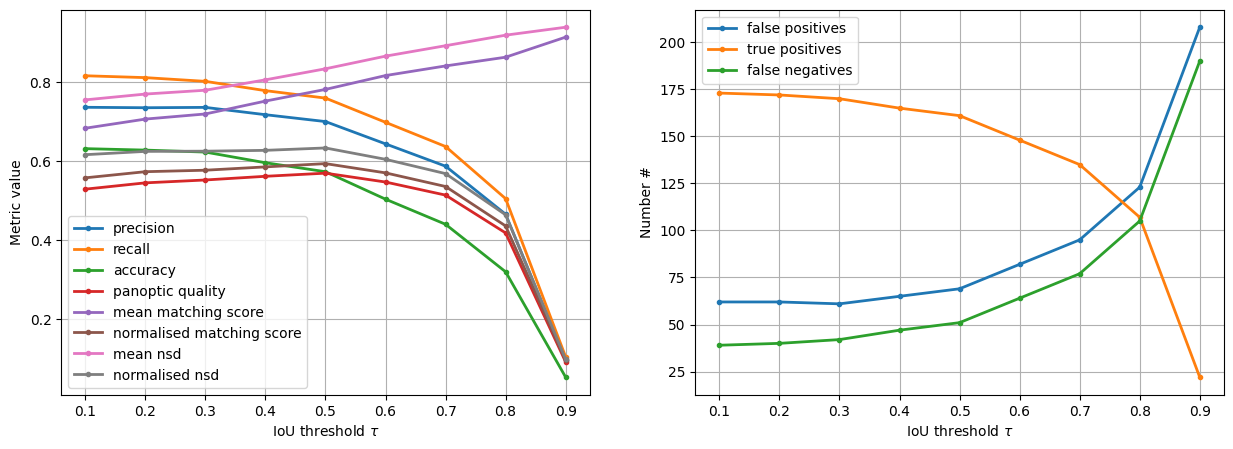
\includegraphics[width=\textwidth]{"images/quantitative_performance_sam.png"}
	\caption[Quantitative performance \texttt{SAM}]{Performance of \texttt{SAM} in terms of the described metrics and ROC metrics.}
	\label{figperfsambase}
\end{figure}
\begin{figure}
	\centering
	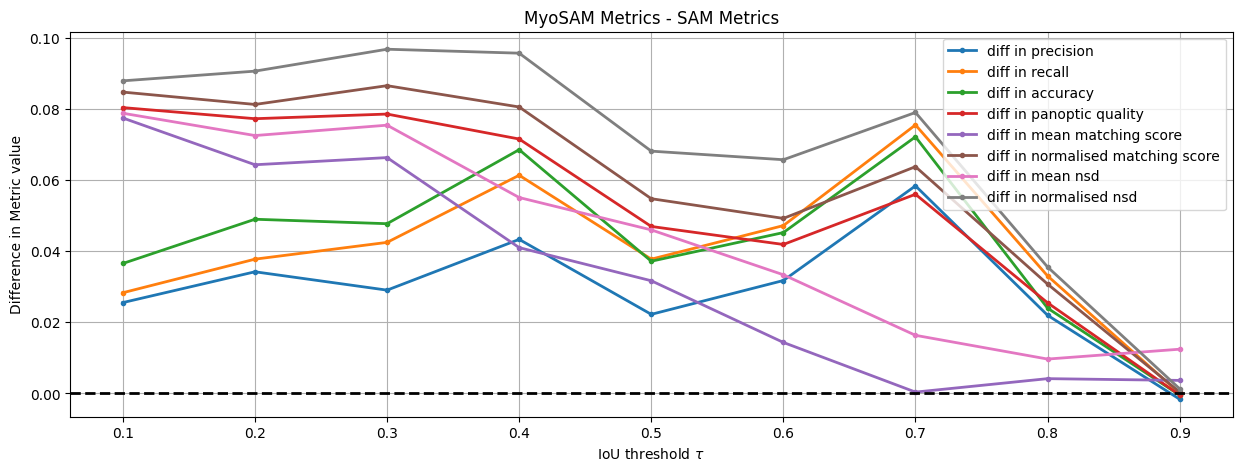
\includegraphics[width=\textwidth]{"images/diff_quantitative_performance_myosam_sam.png"}
	\caption[Difference quantitative performance \texttt{SAM} and \texttt{MyoSAM}]{Performance differences between \texttt{MyoSAM} and \texttt{SAM}.}
	\label{figperfdiffsam}
\end{figure} 


\subsection{Myovision Metrics}
Our research involves segmenting microscopic myotubes and cell nuclei, a process crucial for musculoskeletal researchers and medical practitioners. This segmentation allows for detailed analysis and understanding of myotubes and cell nuclei, providing valuable insights into muscular health and diseases. To support this analysis, our tool has been developed to offer a wide range of metrics in real-time to facilitate a speedy examination with no human error. We offer a total of 31 metrics, divided into image-specific and myotube-specific categories, as detailed in Table~\ref{tabimgspec} and Table~\ref{tabmyospec}.
\subsubsection{Image Specific Metrics}
These metrics primarily count the instances of various musculoskeletal components within an image. Myoblasts are defined as nuclei not contained within a myotube. A nucleus is considered part of a myotube if 95\% or more of its area is inside the myotube. This determination involves a multi-step process, starting with identifying if nuclei centroids are within a myotube's bounding box, then verifying if their centroids are within the myotube's perimeter. We further refine this by converting the relevant myotubes and nuclei into a binary mask to check the percentage of a nucleus's area inside a myotube. However, the masks we create correspond to the size of the myotube’s bounding box instead of the whole image thus optimizing memory usage. Clusters of nuclei within the same myotube are identified by detecting overlaps and creating a graph where nuclei are nodes connected by their overlaps using \ref{hagberg2008exploring}. The number of nodes in this graph represents the number of nuclei in a cluster. Area measurements for myotubes, nuclei, and myoblasts are obtained by counting the pixels within each entity, allowing for conversion to metric scale measurements if the pixel size in the microscopic image is known.
\subsubsection{Myotube Specific Metrics}
These metrics include the predicted Intersection over Union (IoU) and Stability, both built in \texttt{SAM} metrics. Predicted IoU measures the predicted overlap between predicted and reference masks, while Stability assesses the sensitivity of predicted masks to changes in prompts. Pixel activation metrics (such as RGB min, max, mean, median, mode, and standard deviation) provide colour intensity information across three channels. The integrated RGB density metric sums the pixel intensities for each color channel. Shape descriptors like Area, Convex Area, Solidity, Aspect Ratio, Roundness, Perimeter, Feret’s Diameter, and Circularity offer detailed insights into each myotube's physical characteristics. For example, Convex Area is calculated from the area enclosed by the convex hull of a myotube, while Solidity and Roundness measure convexity and circularity, respectively. Feret's Diameters, both minimum and maximum, are derived from linear projections of myotubes using their eigenvectors, measuring their diameter in the directions of minimum and maximum variance. The Instance Fusion Index quantifies the number of nuclei within a specific myotube. Lastly, each myotube is accompanied by cluster information, detailing the number of clusters within a myotube and the number of nuclei in each cluster, along with their indicators.
This comprehensive suite of metrics provided by our \texttt{MyoSAM} tool is designed to facilitate a deeper understanding and analysis of myotubes and their cellular components, offering a robust framework for musculoskeletal research and medical diagnostics.


